%!TEX TS-program = xelatex

% Шаблон документа LaTeX создан в 2018 году
% Алексеем Подчезерцевым
% В качестве исходных использованы шаблоны
% 	Данилом Фёдоровых (danil@fedorovykh.ru) 
%		https://www.writelatex.com/coursera/latex/5.2.2
%	LaTeX-шаблон для русской кандидатской диссертации и её автореферата.
%		https://github.com/AndreyAkinshin/Russian-Phd-LaTeX-Dissertation-Template

\documentclass[a4paper,14pt]{article}

%%% Работа с русским языком
\usepackage[english,russian]{babel}   %% загружает пакет многоязыковой вёрстки
\usepackage{fontspec}      %% подготавливает загрузку шрифтов Open Type, True Type и др.
\defaultfontfeatures{Ligatures={TeX},Renderer=Basic}  %% свойства шрифтов по умолчанию
\setmainfont[Ligatures={TeX,Historic}]{Times New Roman} %% задаёт основной шрифт документа
\setsansfont{Comic Sans MS}                    %% задаёт шрифт без засечек
\setmonofont{Courier New}
\usepackage{indentfirst}
\frenchspacing

\renewcommand{\epsilon}{\ensuremath{\varepsilon}}
\renewcommand{\phi}{\ensuremath{\varphi}}
\renewcommand{\kappa}{\ensuremath{\varkappa}}
\renewcommand{\le}{\ensuremath{\leqslant}}
\renewcommand{\leq}{\ensuremath{\leqslant}}
\renewcommand{\ge}{\ensuremath{\geqslant}}
\renewcommand{\geq}{\ensuremath{\geqslant}}
\renewcommand{\emptyset}{\varnothing}

%%% Дополнительная работа с математикой
\usepackage{amsmath,amsfonts,amssymb,amsthm,mathtools} % AMS
\usepackage{icomma} % "Умная" запятая: $0,2$ --- число, $0, 2$ --- перечисление

%% Номера формул
%\mathtoolsset{showonlyrefs=true} % Показывать номера только у тех формул, на которые есть \eqref{} в тексте.
%\usepackage{leqno} % Нумерация формул слева	

%% Перенос знаков в формулах (по Львовскому)
\newcommand*{\hm}[1]{#1\nobreak\discretionary{}
	{\hbox{$\mathsurround=0pt #1$}}{}}

%%% Работа с картинками
\usepackage{graphicx}  % Для вставки рисунков
\graphicspath{{images/}}  % папки с картинками
\setlength\fboxsep{3pt} % Отступ рамки \fbox{} от рисунка
\setlength\fboxrule{1pt} % Толщина линий рамки \fbox{}
\usepackage{wrapfig} % Обтекание рисунков текстом

%%% Работа с таблицами
\usepackage{array,tabularx,tabulary,booktabs} % Дополнительная работа с таблицами
\usepackage{longtable}  % Длинные таблицы
\usepackage{multirow} % Слияние строк в таблице
\usepackage{float}% http://ctan.org/pkg/float

%%% Программирование
\usepackage{etoolbox} % логические операторы


%%% Страница
\usepackage{extsizes} % Возможность сделать 14-й шрифт
\usepackage{geometry} % Простой способ задавать поля
\geometry{top=20mm}
\geometry{bottom=20mm}
\geometry{left=20mm}
\geometry{right=10mm}
%
%\usepackage{fancyhdr} % Колонтитулы
% 	\pagestyle{fancy}
%\renewcommand{\headrulewidth}{0pt}  % Толщина линейки, отчеркивающей верхний колонтитул
% 	\lfoot{Нижний левый}
% 	\rfoot{Нижний правый}
% 	\rhead{Верхний правый}
% 	\chead{Верхний в центре}
% 	\lhead{Верхний левый}
%	\cfoot{Нижний в центре} % По умолчанию здесь номер страницы

\usepackage{setspace} % Интерлиньяж
\onehalfspacing % Интерлиньяж 1.5
%\doublespacing % Интерлиньяж 2
%\singlespacing % Интерлиньяж 1

\usepackage{lastpage} % Узнать, сколько всего страниц в документе.

\usepackage{soul} % Модификаторы начертания

\usepackage{hyperref}
\usepackage[usenames,dvipsnames,svgnames,table,rgb]{xcolor}
\hypersetup{				% Гиперссылки
	unicode=true,           % русские буквы в раздела PDF
	pdftitle={Автоматизация проектных работ},   % Заголовок
	pdfauthor={Солодянкин А.А.},      % Автор
	pdfsubject={Автоматизация проектных работ},      % Тема
	pdfcreator={Солодянкин А.А.}, % Создатель
	pdfproducer={Солодянкин А.А.}, % Производитель
	pdfkeywords={Автоматизация проектных работ}, % Ключевые слова
	colorlinks=true,       	% false: ссылки в рамках; true: цветные ссылки
	linkcolor=black,          % внутренние ссылки
	citecolor=black,        % на библиографию
	filecolor=magenta,      % на файлы
	urlcolor=black           % на URL
}
\makeatletter 
\def\@biblabel#1{#1. } 
\makeatother
\usepackage{cite} % Работа с библиографией
%\usepackage[superscript]{cite} % Ссылки в верхних индексах
%\usepackage[nocompress]{cite} % 
\usepackage{csquotes} % Еще инструменты для ссылок

\usepackage{multicol} % Несколько колонок

\usepackage{tikz} % Работа с графикой
\usepackage{pgfplots}
\usepackage{pgfplotstable}

% ГОСТ заголовки
\usepackage[font=small]{caption}
%\captionsetup[table]{justification=centering, labelsep = newline} % Таблицы по правобу краю
%\captionsetup[figure]{justification=centering} % Картинки по центру


\newcommand{\tablecaption}[1]{\addtocounter{table}{1}\small \begin{flushright}\tablename \ \thetable\end{flushright}%	
\begin{center}#1\end{center}}

\newcommand{\imref}[1]{рис.~\ref{#1}}

\usepackage{multirow}
\usepackage{spreadtab}
\newcolumntype{K}[1]{@{}>{\centering\arraybackslash}p{#1cm}@{}}


\usepackage{xparse}
\usepackage{fancyvrb}

\RecustomVerbatimCommand{\VerbatimInput}{VerbatimInput}
{
	fontsize=\footnotesize    
}

\newcolumntype{?}[1]{!{\vrule width #1}}

\usepackage{tocloft}
\renewcommand{\cftsecleader}{\cftdotfill{\cftdotsep}}
\begin{document} % конец преамбулы, начало документа
\begin{titlepage}
	\begin{center}
		ПРАВИТЕЛЬСТВО РОССИЙСКОЙ ФЕДЕРАЦИИ \\
 		ФЕДЕРАЛЬНОЕ  ГОСУДАРСТВЕННОЕ АВТОНОМНОЕ \\
		ОБРАЗОВАТЕЛЬНОЕ УЧРЕЖДЕНИЕ ВЫСШЕГО ОБРАЗОВАНИЯ\\
		«НАЦИОНАЛЬНЫЙ ИССЛЕДОВАТЕЛЬСКИЙ УНИВЕРСИТЕТ\\
		«ВЫСШАЯ ШКОЛА ЭКОНОМИКИ»
	\end{center}
	
	\begin{center}
		\textbf{Московский институт электроники и математики}
		
		\textbf{Им. А.Н.Тихонова НИУ ВШЭ}
		
		\vspace{2ex}
		
		\textbf{Департамент компьютерной инженерии}
	\end{center}
	\vspace{1ex}	
	
	\vspace{1ex}
	\begin{center}
		\textbf{Практическая работа №7 \\
			<<Математические модели для решения задач размещения на печатной плате>> \\
			по курсу <<Автоматизация проектных работ>>\\
	}
	\end{center}	

	\vspace{2ex}
	\vfill
	
	\vspace{2ex}
	
	\begin{flushright}
		\textbf{Выполнил:}
		
		\vspace{2ex}
		
		Студент группы БИВ174
		
		\vspace{2ex}
		
		Солодянкин Андрей Александрович
		
		\vspace{2ex}
		
		\textbf{Проверил:}
		
		\vspace{2ex}
		
		Новиков Константин Викторович
	\end{flushright}

	\vspace{5ex}
	\begin{center}
		Москва \the\year \, г.
	\end{center}
	
\end{titlepage}
\addtocounter{page}{1}
\tableofcontents
\pagebreak

\section{Задание}

Экспериментально получить вольт – амперную характеристику (ВАХ) полупроводникового диода.
Исследовать влияние температуры на характеристики p-n диодов.


\section{Краткие теоретические сведения}

\subsection{Что такое идеальный диод?}
Основная задача обычного выпрямительного диода – проводить электрический ток в одном направлении, и не пропускать его в обратном. 
Следовательно, идеальный диод должен быть очень хорошим проводником с нулевым сопротивлением при прямом подключении напряжения (плюс - к аноду, минус - к катоду), и абсолютным изолятором с бесконечным сопротивлением при обратном.
Вот так это выглядит на графике:

\begin{figure}[H]
	\centering
	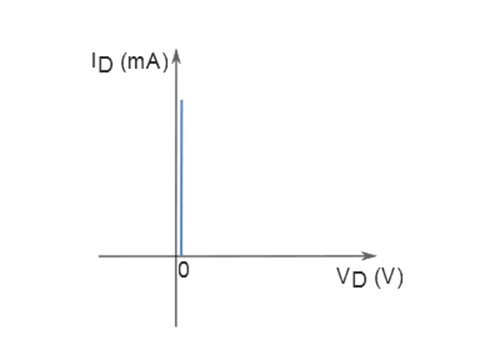
\includegraphics[width=0.5\linewidth]{image/intro_001}
	\caption{График зависимости тока от напряжения на идеальном диоде}
	\label{fig:intro001}
\end{figure}

Такая модель диода используется в случаях, когда важна только логическая функция прибора. Например, в цифровой электронике.

\subsection{ВАХ реального полупроводникового диода}

Однако на практике, в силу своей полупроводниковой структуры, настоящий диод обладает рядом недостатков и ограничений по сравнению с идеальным диодом. 
Это можно увидеть на графике, приведенном ниже.

\begin{figure}[H]
	\centering
	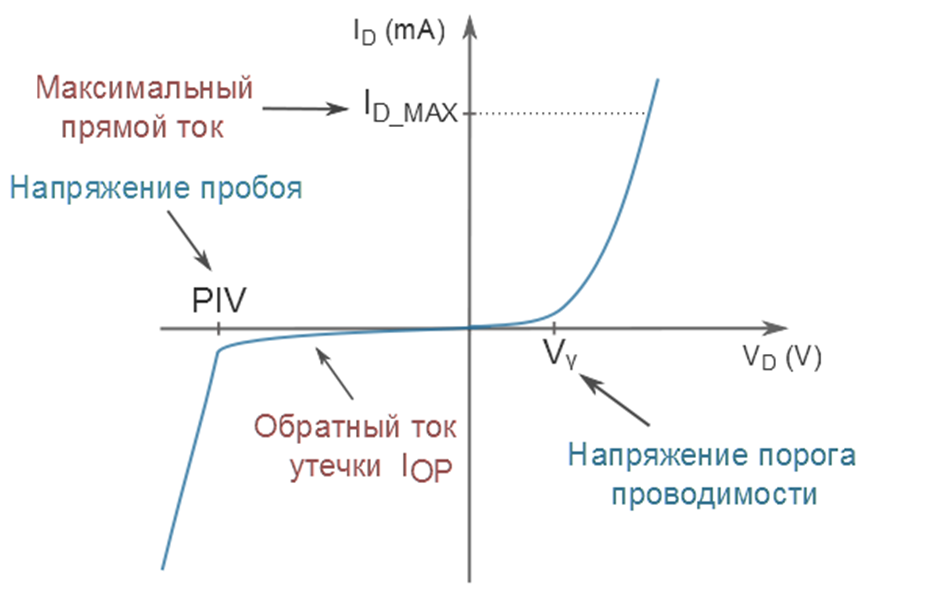
\includegraphics{image/intro_002}
	\caption{Зависимость тока от напряжения в настоящем диоде}
	\label{fig:intro002}
\end{figure}

\subsubsection{$V_{\gamma}$(гамма) -- напряжение порога проводимости.}

При прямом включении напряжение на диоде должно достигнуть определенного порогового значения - $V_{\gamma}$. 
Это напряжение, при котором PN-переход в полупроводнике открывается достаточно, чтобы диод начал хорошо проводить ток. 
До того как напряжение между анодом и катодом достигнет этого значения, диод является очень плохим проводником. 
$V_{\gamma}$ у кремниевых приборов примерно 0.7V, у германиевых – около 0.3V.

\subsubsection{$I_{D\_MAX}$ -- максимальный ток через диод при прямом включении.}

При прямом включении полупроводниковый диод способен выдержать ограниченную силу тока $I_{D\_MAX}$. 
Когда ток через прибор превышает этот предел, диод перегревается. 
В результате разрушается кристаллическая структура полупроводника, и прибор становится непригодным. 
Величина данной силы тока сильно колеблется в зависимости от разных типов диодов и их производителей.

\subsubsection{$I_{OP}$ -- обратный ток утечки.}

При обратном включении диод не является абсолютным изолятором и имеет конечное сопротивление, хоть и очень высокое. 
Это служит причиной образования тока утечки или обратного тока $I_{OP}$. 
Ток утечки у германиевых приборов достигает до 200 µА, у кремниевых до нескольких десятков nА. 
Самые последние высококачественные кремниевые диоды с предельно низким обратным током имеют этот показатель около 0.5 nA.

\subsubsection{$PIV$ (Peak Inverse Voltage) -- Напряжение пробоя.}

При обратном включении диод способен выдерживать ограниченное напряжение – напряжение пробоя $PIV$.
Если внешняя разность потенциалов превышает это значение, диод резко понижает свое сопротивление и превращается в проводник. 
Такой эффект нежелательный, так как диод должен быть хорошим проводником только при прямом включении. 
Величина напряжения пробоя колеблется в зависимости от разных типов диодов и их производителей.

\subsubsection{Паразитическая емкость PN-перехода.}

Даже если на диод подать напряжение значительно выше $V_{\gamma}$, он не начнет мгновенно проводить ток.
Причиной этому является паразитическая емкость PN перехода, на наполнение которой требуется определенное время. 
Это сказывается на частотных характеристиках прибора.

\begin{figure}[H]
	\centering
	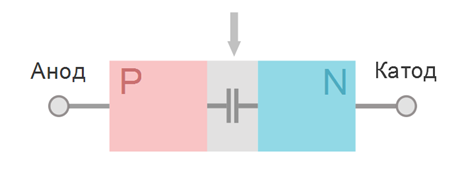
\includegraphics[width=0.7\linewidth]{image/intro_003}
	\caption{Паразитическая емкость}
	\label{fig:intro003}
\end{figure}

\subsection{Приближенные модели диодов}

В большинстве случаев, для расчетов в электронных схемах, не используют точную модель диода со всеми его характеристиками. Нелинейность этой функции слишком усложняет задачу. Предпочитают использовать, так называемые, приближенные модели.

\subsubsection{Приближенная модель диода <<идеальный диод + $V_{\gamma}$>>}

Самой простой и часто используемой является приближенная модель первого уровня. Она состоит из идеального диода и, добавленного к нему, напряжения порога проводимости $V_{\gamma}$.

\begin{figure}[H]
	\centering
	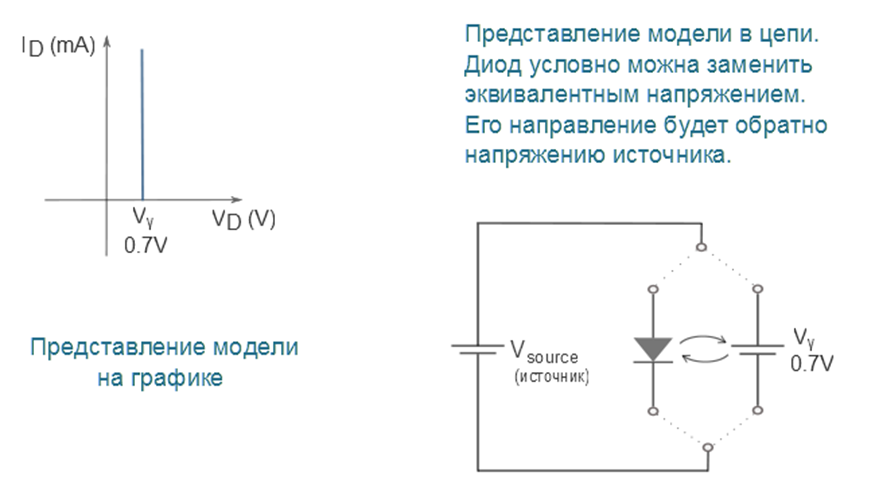
\includegraphics[width=0.7\linewidth]{image/intro_004}
	\caption{Приближенная модель диода <<идеальный диод + $V_{\gamma}$>>}
	\label{fig:intro004}
\end{figure}

\subsubsection{Приближенная модель диода <<идеальный диод + $V_{\gamma} + r_D$>>}

Иногда используют чуть более сложную и точную приближенную модель второго уровня. В этом случае добавляют к модели первого уровня внутреннее сопротивление диода, преобразовав его функцию из экспоненты в линейную.

\begin{figure}[H]
	\centering
	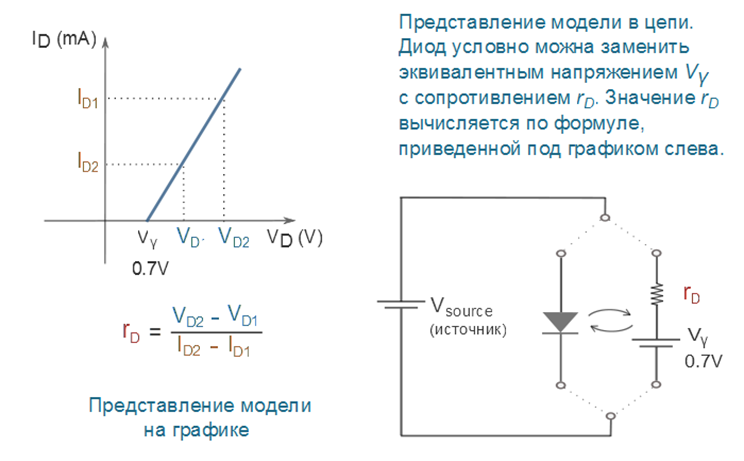
\includegraphics[width=0.7\linewidth]{image/intro_005}
	\caption{Приближенная модель диода <<идеальный диод + $V_{\gamma} + r_D$>>}
	\label{fig:intro005}
\end{figure}


\section{Выполнение работы}

На рис.~\ref{fig:temp_25} изображена ВАХ диода при значении тока $I_o = 1.5 uA$.
По информации из таблицы, данный диод -- КД204А.
На рис.~\ref{fig:temp_0}~и~\ref{fig:temp_75} представлены ВАХ диода при $T=0^{\circ} C$ и $T=75^{\circ} C$ соответственно.
При увеличении температуры можно наблюдать, как график ВАХ сдвигается вправо.
Это происходит по причине уменьшения контактной разности потенциалов, возрастания энергии основных носителей заряда, расту диффузионной составляющей тока и увеличению прямого тока. 
	
\begin{figure}[H]
	\centering
	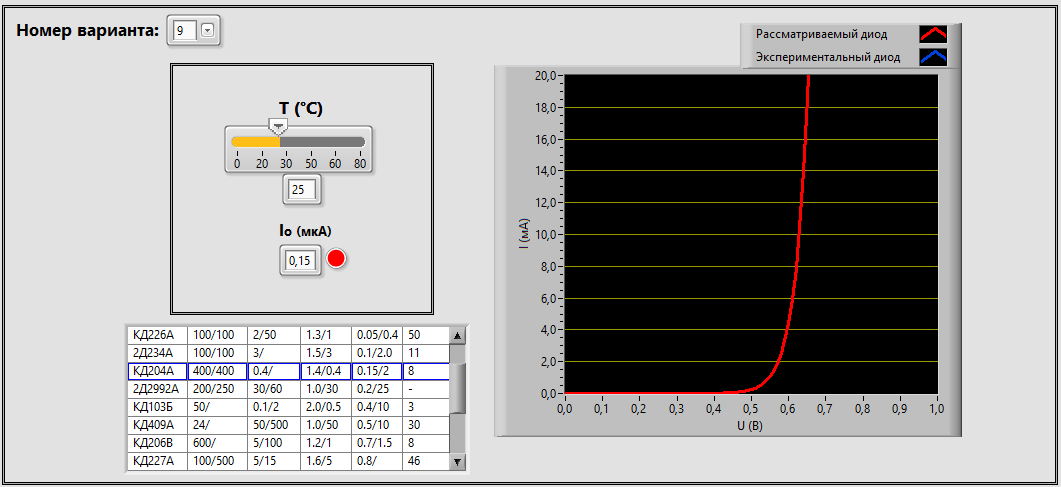
\includegraphics[width=\linewidth]{image/temp_25}
	\caption{ВАХ диода при $T=25^{\circ} C$}
	\label{fig:temp_25}
\end{figure}


\begin{figure}[H]
	\centering
	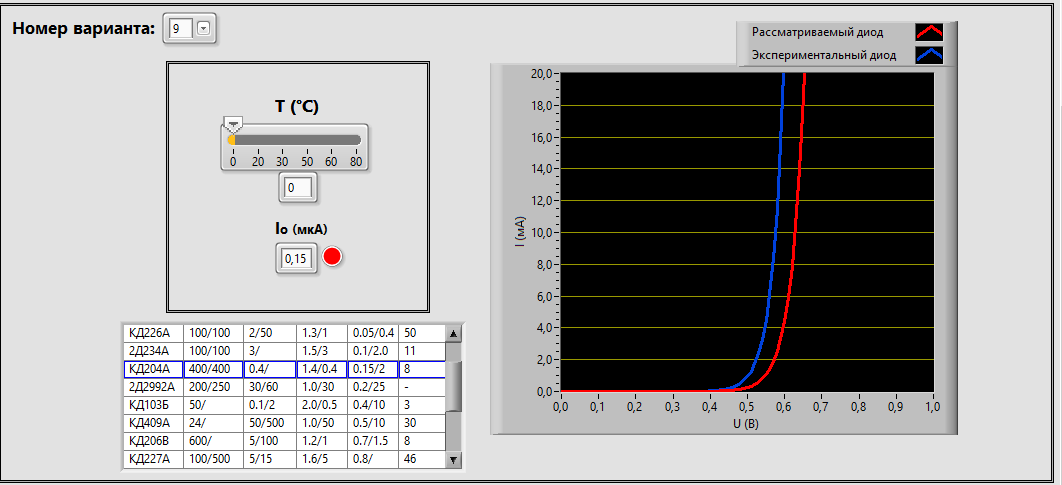
\includegraphics[width=\linewidth]{image/temp_0}
	\caption{ВАХ диода при $T=0^\circ C$}
	\label{fig:temp_0}
\end{figure}

\begin{figure}[H]
	\centering
	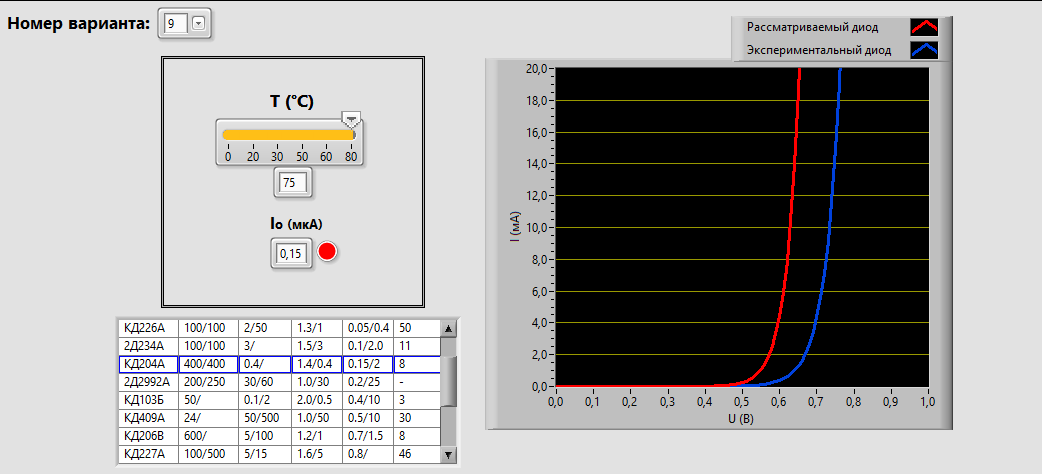
\includegraphics[width=\linewidth]{image/temp_75}
	\caption{ВАХ диода при $T=75^\circ C$}
	\label{fig:temp_75}
\end{figure}
\section{Выводы по работе}

В ходе выполнения лабораторной работы было получено экспериментальным путем ВАХ полупроводникового диода. Найдено значение обратного тока, при котором возможно совпадение графиков ВАХ экспериментального и рассматриваемого диода. Исследовано влияние температуры на вольтамперные характеристики диодов.

\section{Контрольные вопросы}

\begin{enumerate}
	\item Что такое полупроводниковый диод.
	
	Полупроводниковый диод -- это полупроводниковый прибор, во внутренней структуре которого сформирован один p-n-переход.
	
	\item Влияние температуры на характеристики p-n диодов.
	
	При большей температуре p-n-перехода тот же прямой ток достигается при меньшем смещении.
	
	\item Способ снятия ВАХ диодов с помощью амперметра и вольтметра.
	
	Вольтметр подключается параллельно диоду, а амперметр -- последовательно.
	
	\item Работа p-n перехода при прямом и обратном включении.
	
	При прямом включении p-n-перехода внешнее напряжение создает в переходе поле, которое противоположно по направлению внутреннему диффузионному полю. 
	Напряженность результирующего поля падает, что сопровождается сужением запирающего слоя. 
	В результате этого большое количество основных носителей зарядов получает возможность диффузионно переходить в соседнюю область. 
	Диффузионный ток зависит от высоты потенциального барьера и по мере его снижения увеличивается экспоненциально. 
	Повышенная диффузия носителей зарядов через переход приводит к повышению концентрации дырок в области n-типа и электронов в области p-типа.
	Такое повышение концентрации неосновных носителей вследствие влияния внешнего напряжения, приложенного к переходу, называется инжекцией неосновных носителей. 
	Неравновесные неосновные носители диффундируют вглубь полупроводника и нарушают его электронейтральность. 
	Восстановление нейтрального состояния полупроводника происходит за счет поступления носителей зарядов от внешнего источника. 
	Это является причиной возникновения тока во внешней цепи, называемого прямым.
	
	При включении p-n-перехода в обратном направлении внешнее обратное напряжение создает электрическое поле, совпадающее по направлению с диффузионным, что приводит к росту потенциального барьера и увеличению ширины запирающего слоя. 
	Все это уменьшает диффузионные токи основных носителей. 
	Для неосновных носителей поле в p-n-переходе остается ускоряющим, и поэтому дрейфовый ток не изменяется. Таким образом, через переход будет протекать результирующий ток, определяемый в основном током дрейфа неосновных носителей. 
	Поскольку количество дрейфующих неосновных носителей не зависит от приложенного напряжения (оно влияет только на их скорость), то при увеличении обратного напряжения ток через переход стремится к предельному значению $I_S$, которое называется током насыщения.

	\item Основные параметры диода.
	
	\begin{itemize}
      	\item $U_{obr.max.}$ -- максимально-допустимое постоянное обратное напряжение диода;
		
		\item $U_{obr.i.max.}$ -- максимально-допустимое импульсное обратное напряжение диода;
		
		\item $I_{f.max.}$ -- максимальный средний прямой ток за период;
		
		\item $I_{f.i.max.}$ -- максимальный импульсный прямой ток за период;
		
		\item $I_{over.max.}$ -- ток перегрузки выпрямительного диода;
		
		\item $f_{max}$ -- максимально-допустимая частота переключения диода;
		
		\item $f_{work}$ -- рабочая частота переключения диода;
		
		\item $U_{f} | I_{f}$ -- постоянное прямое напряжения диода при токе Iпр;
		
		\item $I_{obr}$ -- постоянный обратный ток диода;
		
		\item $T_{k.max.}$ -- максимально-допустимая температура корпуса диода;
		
		\item $T_{p.max.}$ -- максимально-допустимая температура перехода диода.
	\end{itemize}
	
	
	\item ВАХ идеального диода.
	
	\begin{figure}[H]
		\centering
		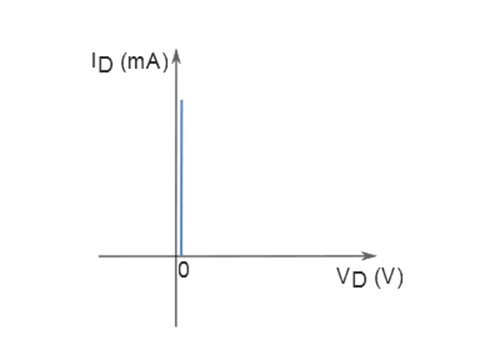
\includegraphics[width=0.5\linewidth]{image/intro_001}
		\caption{График зависимости тока от напряжения на идеальном диоде}
	\end{figure}
\end{enumerate}

\end{document} % конец документа